\documentclass[12pt]{article}
\usepackage[table]{xcolor}
\usepackage[shortlabels]{enumitem}
\usepackage{tabularx,xltabular}
\usepackage{graphicx}
\usepackage{hyperref}
\usepackage{verbatim}
\usepackage{geometry}
\usepackage{ulem}
\usepackage[official]{eurosym}
\usepackage{tikz}
\usetikzlibrary{arrows,backgrounds,calc,decorations.markings,patterns,3d,positioning,fit,angles, quotes}
\usepackage{pgfplots}
\pgfplotsset{compat = newest}
\usetikzlibrary{fit}
\newcommand\addvmargin[1]{
\usetikzlibrary{arrows}
\node[fit=(current bounding box),inner ysep=#1,inner xsep=0]{};}
\usepackage{cancel}
\usepackage{fontspec}
\usepackage{array}  
\geometry{a4paper, top=2cm, left=2cm, right=2cm, bottom=2cm, headsep=1cm}
\usepackage{tabu}
\usepackage{pst-node}
\usepackage{colortbl}
\usepackage{array}
\usepackage{german}
\setlength\parindent{0pt}
\newcolumntype{?}{!{\vrule width 1pt}}
\usepackage{makecell}
\renewcommand{\arraystretch}{2.5}
\usepackage{pbox}
\usepackage{amssymb}
\usepackage{amsmath}
\usepackage{booktabs}
\newcolumntype{L}[1]{>{\raggedright\let\newline\\\arraybackslash\hspace{0pt}}m{#1}}
\newcolumntype{C}[1]{>{\centering\let\newline\\\arraybackslash\hspace{0pt}}m{#1}}
\newcolumntype{R}[1]{>{\raggedleft\let\newline\\\arraybackslash\hspace{0pt}}m{#1}}
\begin{document}
\rightline{Datum: 08.12.2023}
\centerline{{\Large Üben für die Arbeit}} 
\vspace{1cm}
\noindent \\


\begin{xltabular}{\textwidth}{|C{0.75cm}|X|}
\arrayrulecolor{black}\hline
a)&Setze für die Variabel x den Wert 8 ein und berechne den Wert des Terms:$$x - 4 \cdot x$$
\\\hline
b)&Setze für die Variabel b den Wert 5 ein und berechne den Wert des Terms:$$4 + 4 \cdot b$$
\\\hline
c)&Vereinfache:$$2x - x - x=?$$
\\\hline
d)&Vereinfache:$$4 - 2b + 3 + 5=?$$
\\\hline
e)&Berechne die Variable $$2\cdot b-11=-5$$
\\\hline
f)&Berechne die Variable $$5\cdot a-8=12$$
\\\hline
g)&\pbox{6cm}{Bestimme den Umfang und die Fläche von: \\\tikzstyle{background grid}=[draw, black!15,step=.5cm]
\noindent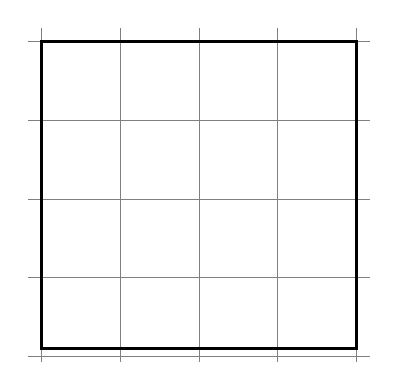
\begin{tikzpicture}[show background grid]
\draw[black, very thick] (0cm,0.1cm) rectangle (4cm,4cm);
\end{tikzpicture}}
\\\hline
h)&\pbox{5cm}{
Berechne den Flächeninhalt von:\\
\tikzstyle{background grid}=[draw, black!15,step=.5cm]
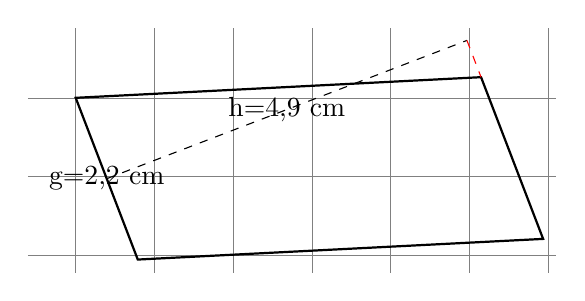
\begin{tikzpicture}[show background grid]
\draw[thick,black,rotate=291] (0,0) -- node{g=2,2 cm} ++(2.2,0) -- ++(1.6,4.9) -- ++(-2.2,0) --cycle;
\draw[dashed,black,rotate=291] (1.1,0)  -- node{h=4,9 cm} ++(0,4.9);
\draw[dashed,black,rotate=291,red] (1.1,4.9)  -- ++(0.5,0);
\end{tikzpicture}
}
\\\hline
i)&\pbox{5cm}{
Berechne den Flächeninhalt von:\\
\tikzstyle{background grid}=[draw, black!15,step=.5cm]
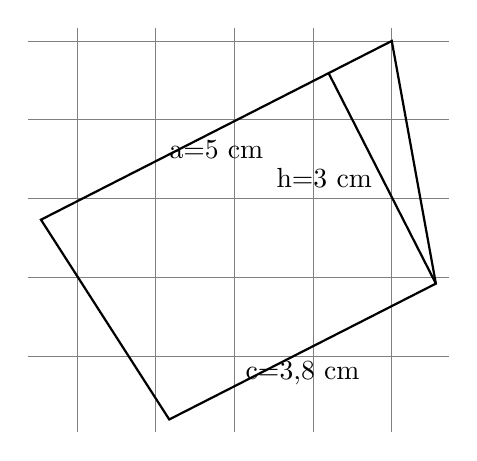
\begin{tikzpicture}[show background grid]
\draw[thick,black,rotate=207] (0,0) -- node[below]{a=5 cm} ++(5.0,0) -- ++(-0.3,3.0) --node[below]{c=3,8 cm} ++(-3.8,0) --cycle;
\draw[thick,black,rotate=207] (0.9000000000000001,0) --node[left]{h=3 cm}  ++(0,3.0);
\end{tikzpicture}
}
\\\hline
j)&\pbox{5cm}{
Berechne den Flächeninhalt von:\\
\tikzstyle{background grid}=[draw, black!15,step=.5cm]
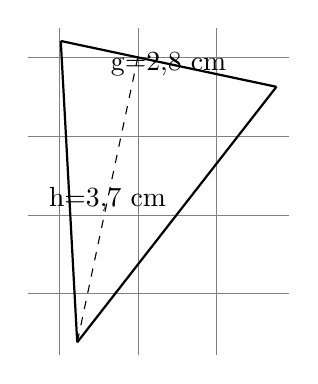
\begin{tikzpicture}[show background grid]
\draw[thick,black] (168:-1.7999999999999998) -- node{g=2,8 cm} (168:1.0);
\draw[thick,black] (168:-1.7999999999999998)  -- (258:3.7);
\draw[thick,black] (168:1.0)  -- (258:3.7);
\draw[dashed,black] (0,0)  -- node{h=3,7 cm} (258:3.7);
\draw[dashed,black] (0,0)  -- (168:-1.7999999999999998);
\end{tikzpicture}
}
\\\hline
k)&\pbox{5cm}{
Berechne den Flächeninhalt von:\\
\tikzstyle{background grid}=[draw, black!15,step=.5cm]
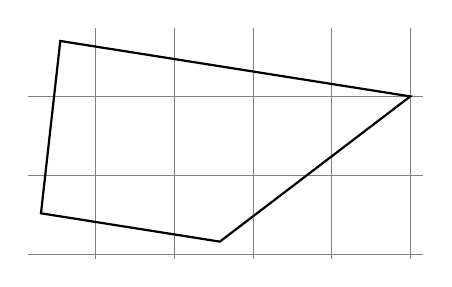
\begin{tikzpicture}[show background grid]
\draw[thick,black,rotate=171] (0,0) -- node[below]{} ++(4.5,0) -- ++(-0.1,2.2) --node[below]{} ++(-2.3,0) --cycle;
\end{tikzpicture}
}
\\\hline
l)&\pbox{5cm}{
Berechne den Flächeninhalt von:\\
\tikzstyle{background grid}=[draw, black!15,step=.5cm]
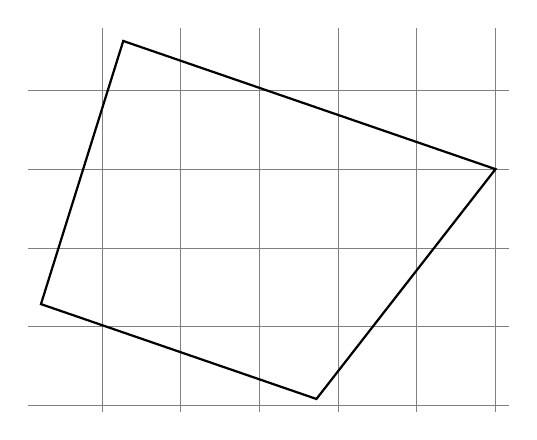
\begin{tikzpicture}[show background grid]
\draw[thick,black,rotate=161] (0,0) -- node[below]{} ++(5.0,0) -- ++(-0.1,3.5) --node[below]{} ++(-3.7,0) --cycle;
\end{tikzpicture}
}
\\\hline
m)&Stelle die Umfangsformel des Parallelogramm nach der fehlenden Seite um und berechne diese und den Flächeninhalt für $u=36~cm$, $a=9,2~cm$ und $h_b=1 cm$.
\\\hline
n)&Stelle die Flächenformel des Rechtecks nach der fehlenden Seite um und berechne diese und den Umfang für $A=4,1~cm^2$ und $b=1~cm$.
\\\hline
\end{xltabular}
\vspace{0.5cm}
\newpage
\rightline{Datum: 08.12.2023}
\centerline{{\large Lösungen Üben für die Arbeit}} 
\vspace{0.5cm}

\begin{xltabular}{\textwidth}{|C{0.75cm}|X|C{0.75cm}|X|}
\arrayrulecolor{black}\hline
a)&$\begin{aligned}
\textcolor{red}{x=8} & \rightarrow\\
x - 4 \cdot x=&\textcolor{red}{8} - 4 \cdot \textcolor{red}{8}=-24\\
\end{aligned}$
&
b)&$\begin{aligned}
\textcolor{red}{b=5} & \rightarrow\\
4 + 4 \cdot b=&4 + 4 \cdot \textcolor{red}{5}=24\\
\end{aligned}$
\\\hline
c)&$2x - x - x=0$
&
d)&$4 - 2b + 3 + 5=12 - 2b$
\\\hline
e)&\begingroup\setlength{\jot}{-0.03cm}
\tikzstyle{background grid}=[draw, black!15,step=.5cm]
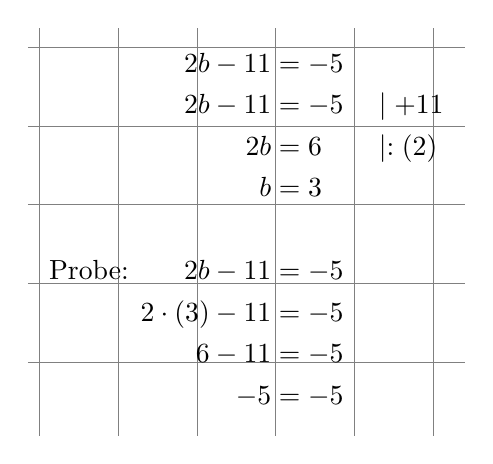
\begin{tikzpicture}[show background grid]
\node[below right] at (0,0.1) {
$\begin{aligned}
2b-11 &=-5& &  \\
2b - 11 &=-5& & \mid + 11\\
2b &=6& & \mid :\left(2\right)\\
b &=3& & 
\\
\\
\mbox{Probe:}\qquad 2b-11 &=-5& &  \\
2\cdot \left(3\right)-11 &=-5& &  \\
6-11 &=-5& &  \\
-5 &=-5& &  \\
\end{aligned}$};
\end{tikzpicture}
\endgroup
&
f)&\begingroup\setlength{\jot}{-0.03cm}
\tikzstyle{background grid}=[draw, black!15,step=.5cm]
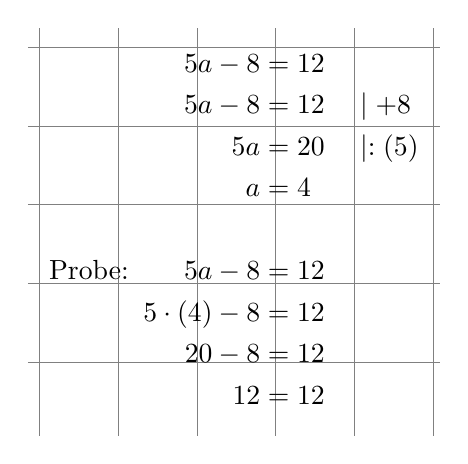
\begin{tikzpicture}[show background grid]
\node[below right] at (0,0.1) {
$\begin{aligned}
5a-8 &=12& &  \\
5a - 8 &=12& & \mid + 8\\
5a &=20& & \mid :\left(5\right)\\
a &=4& & 
\\
\\
\mbox{Probe:}\qquad 5a-8 &=12& &  \\
5\cdot \left(4\right)-8 &=12& &  \\
20-8 &=12& &  \\
12 &=12& &  \\
\end{aligned}$};
\end{tikzpicture}
\endgroup
\\\hline
g)&\pbox{6cm}{$U=2\cdot a+2\cdot b$ \\ $U=2\cdot4cm+2\cdot4cm=16cm$ \\$A=a\cdot b$ \\ $A=4\cdot4=16cm^2$ \\\tikzstyle{background grid}=[draw, black!15,step=.5cm]
\noindent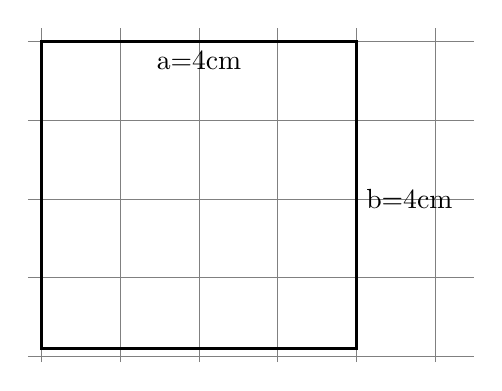
\begin{tikzpicture}[show background grid]
\draw[black, very thick] (0cm,0.1cm) rectangle (4cm,4cm);
\draw (2.0cm,4cm) node[below]{a=4cm}; 
\draw (4cm,2.0cm) node[right]{b=4cm}; 
\end{tikzpicture}}
&
h)&\pbox{5cm}{
$\begin{aligned}
geg.: g&=2,2 cm \\
   h&=4,9 cm \\
ges.: A&=? \\
A&=g\cdot h \\
&=2,2\cdot 4,9 \\
\makebox[0pt][l]{\uuline{\phantom{$A=10,78~cm^2$} } }
A&=10,78~cm^2
\end{aligned}$
\tikzstyle{background grid}=[draw, black!15,step=.5cm]
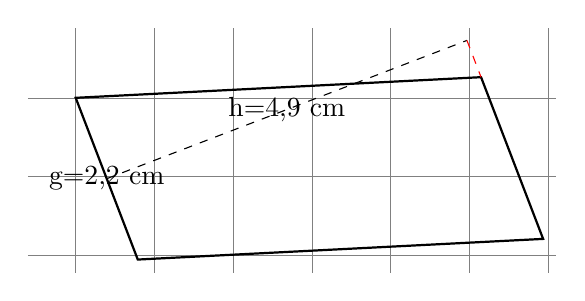
\begin{tikzpicture}[show background grid]
\draw[thick,black,rotate=291] (0,0) -- node{g=2,2 cm} ++(2.2,0) -- ++(1.6,4.9) -- ++(-2.2,0) --cycle;
\draw[dashed,black,rotate=291] (1.1,0)  -- node{h=4,9 cm} ++(0,4.9);
\draw[dashed,black,rotate=291,red] (1.1,4.9)  -- ++(0.5,0);
\end{tikzpicture}
}
\\\hline
i)&\pbox{5cm}{
\tikzstyle{background grid}=[draw, black!15,step=.5cm]
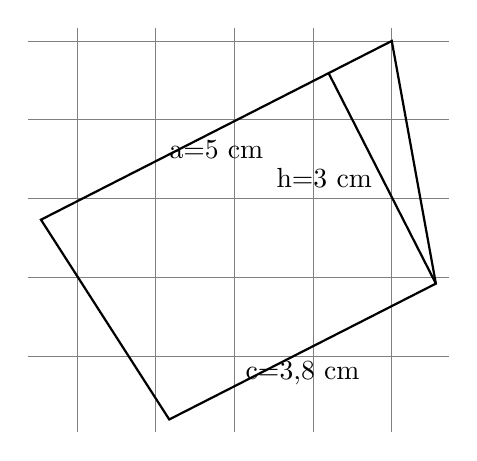
\begin{tikzpicture}[show background grid]
\draw[thick,black,rotate=207] (0,0) -- node[below]{a=5 cm} ++(5.0,0) -- ++(-0.3,3.0) --node[below]{c=3,8 cm} ++(-3.8,0) --cycle;
\draw[thick,black,rotate=207] (0.9000000000000001,0) --node[left]{h=3 cm}  ++(0,3.0);
\end{tikzpicture}
$\begin{aligned}
geg.: a&=5 cm \\
   c&=3,8 cm \\
   h&=3 cm \\
ges.: A&=? \\
A&=\frac{a+c}{2}\cdot h \\
&=\frac{5+3,8}{2}\cdot3\\
\makebox[0pt][l]{\uuline{\phantom{$A=13,2~cm^2$} } }
A&=13,2~cm^2
\end{aligned}$
}
&
j)&\pbox{5cm}{
$\begin{aligned}
geg.: g&=2,8 cm \\
   h&=3,7 cm \\
ges.: A&=? \\
A&=\frac{g \cdot h}{2} \\
&=2,8 \cdot \frac{3,7}{2}\\
\makebox[0pt][l]{\uuline{\phantom{$A=5,18~cm^2$} } }
A&=5,18~cm^2
\end{aligned}$
\tikzstyle{background grid}=[draw, black!15,step=.5cm]
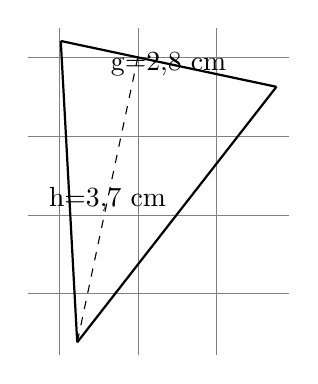
\begin{tikzpicture}[show background grid]
\draw[thick,black] (168:-1.7999999999999998) -- node{g=2,8 cm} (168:1.0);
\draw[thick,black] (168:-1.7999999999999998)  -- (258:3.7);
\draw[thick,black] (168:1.0)  -- (258:3.7);
\draw[dashed,black] (0,0)  -- node{h=3,7 cm} (258:3.7);
\draw[dashed,black] (0,0)  -- (168:-1.7999999999999998);
\end{tikzpicture}
}
\\\hline
k)&\pbox{5cm}{
\tikzstyle{background grid}=[draw, black!15,step=.5cm]
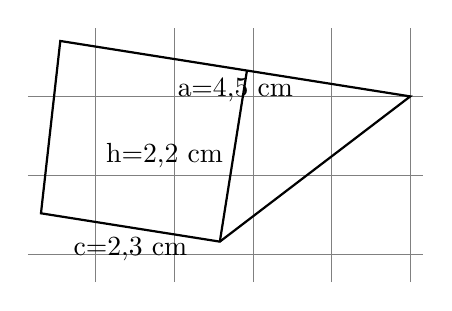
\begin{tikzpicture}[show background grid]
\draw[thick,black,rotate=171] (0,0) -- node[below]{a=4,5 cm} ++(4.5,0) -- ++(-0.1,2.2) --node[below]{c=2,3 cm} ++(-2.3,0) --cycle;
\draw[thick,black,rotate=171] (2.1,0) --node[left]{h=2,2 cm}  ++(0,2.2);
\end{tikzpicture}
$\begin{aligned}
geg.: a&=4,5 cm \\
   c&=2,3 cm \\
   h&=2,2 cm \\
ges.: A&=? \\
A&=\frac{a+c}{2}\cdot h \\
&=\frac{4,5+2,3}{2}\cdot2,2\\
\makebox[0pt][l]{\uuline{\phantom{$A=7,48~cm^2$} } }
A&=7,48~cm^2
\end{aligned}$
}
&
l)&\pbox{5cm}{
\tikzstyle{background grid}=[draw, black!15,step=.5cm]
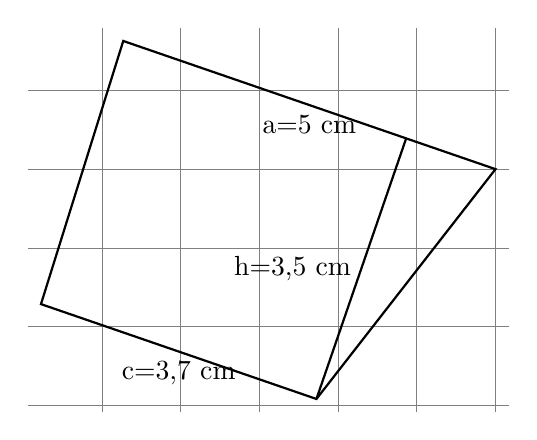
\begin{tikzpicture}[show background grid]
\draw[thick,black,rotate=161] (0,0) -- node[below]{a=5 cm} ++(5.0,0) -- ++(-0.1,3.5) --node[below]{c=3,7 cm} ++(-3.7,0) --cycle;
\draw[thick,black,rotate=161] (1.1999999999999997,0) --node[left]{h=3,5 cm}  ++(0,3.5);
\end{tikzpicture}
$\begin{aligned}
geg.: a&=5 cm \\
   c&=3,7 cm \\
   h&=3,5 cm \\
ges.: A&=? \\
A&=\frac{a+c}{2}\cdot h \\
&=\frac{5+3,7}{2}\cdot3,5\\
\makebox[0pt][l]{\uuline{\phantom{$A=15,22~cm^2$} } }
A&=15,22~cm^2
\end{aligned}$
}
\\\hline
m)&\tikzstyle{background grid}=[draw, black!15,step=.5cm]
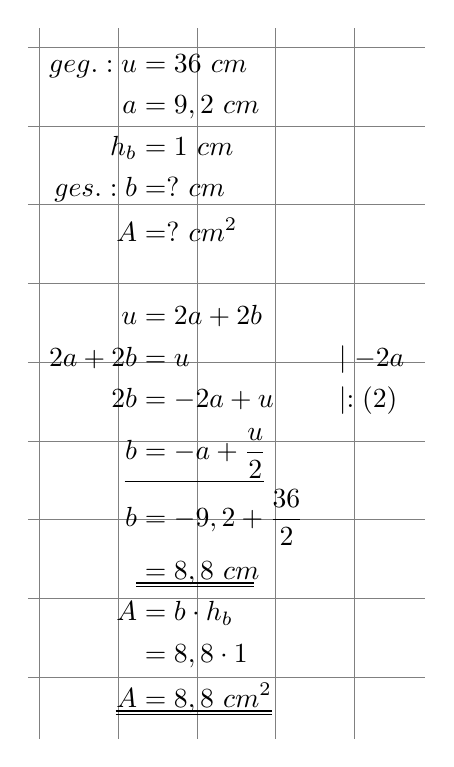
\begin{tikzpicture}[show background grid]
\node[below right] at (0,0.1) {
$\begin{aligned}
geg.: u &=36~cm& & \\
  a &=9,2~cm& & \\
 h_b &=1~cm& & \\
ges.: b &=?~cm& & \\
A &=?~cm^2& & \\
& & & \\
u &=2a+2b& & \\
2a + 2b &=u& & \mid -2a \\
2b &=-2a + u& & \mid :(2)\\
\makebox(0pt,-0.25cm)[l]{\uline{\phantom{$b =-a +{{\frac{ u}{2}}}  \\$}}}
b &=-a +{{\frac{ u}{2}}}& & \\
b&=-9,2+\frac{36}{2}& & \\
\makebox[0pt][l]{\uuline{\phantom{$=8,8~cm  \\$}}}
&=8,8~cm& & \\
A&=b\cdot h_b & & \\
&=8,8\cdot1& & \\
\makebox[0pt][l]{\uuline{\phantom{$A=8,8~cm^2     \\$}}}
A&=8,8~cm^2   & & \\
\end{aligned}$};
\end{tikzpicture}
&
n)&\tikzstyle{background grid}=[draw, black!15,step=.5cm]
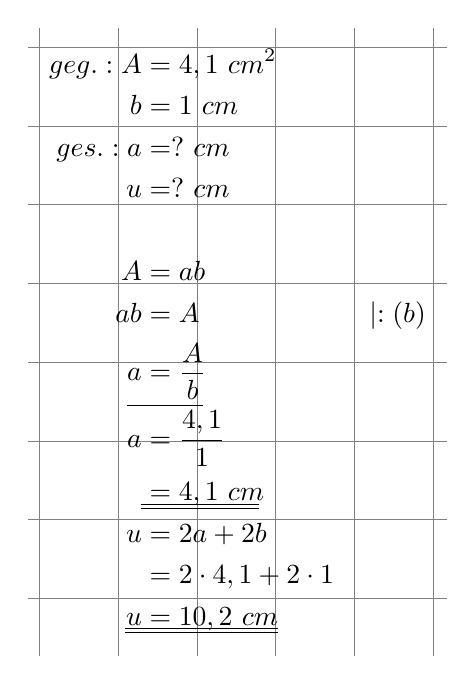
\begin{tikzpicture}[show background grid]
\node[below right] at (0,0.1) {
$\begin{aligned}
geg.: A &=4,1~cm^2& & \\
  b &=1~cm& & \\
ges.: a &=?~cm& & \\
u &=?~cm& & \\
& & & \\
A &=ab& & \\
ab &=A& & \mid :(b)\\
\makebox(0pt,-0.25cm)[l]{\uline{\phantom{$a ={{\frac{A}{b}}}  \\$}}}
a &={{\frac{A}{b}}}& & \\
a&=\frac{4,1}{1}& & \\
\makebox[0pt][l]{\uuline{\phantom{$=4,1~cm  \\$}}}
&=4,1~cm& & \\
u&=2a+2b & & \\
&=2\cdot4,1+2\cdot1& & \\
\makebox[0pt][l]{\uuline{\phantom{$u=10,2~cm     \\$}}}
u&=10,2~cm   & & \\
\end{aligned}$};
\end{tikzpicture}
\\\hline
\end{xltabular}
\vspace{0.5cm}
\end{document}